\section{Michał Karpierz}
\textbf{Równoważność masy i energii} to koncepcja, według której masa obiektu lub układu jest miarą zawartej w nim energii. Koncepcja ta wywodzi się ze \emph{szczególnej teorii względności}.

Pewne obiekty fizyczne (tzw. ciała fizyczne) i układy fizyczne (niekoniecznie złożone z ciał fizycznych), o niezerowej masie spoczynkowej, mają niezerową tzw. energię spoczynkową. Energia ta wyraża się wzorem:

$$E=mc^2$$

gdzie:
\begin{itemize}
    \item $E$ - energia spoczynkowa,
    \item $c$ - prędkość światła w próżni,
    \item $m$ - masa spoczynkowa.
\end{itemize}
\begin{figure}[]
    \centering
    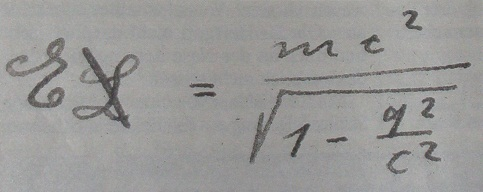
\includegraphics[width=0.75\textwidth, inner]{pictures/E_mc_2_IMG_0859.jpg}
    \caption{Równanie równoważności masy i energii}
    \label{fig:emc}
\end{figure}
Notatka widoczna na zdjęciu nr \ref{fig:emc} zostałą sporządzona w 1912 r przez Alberta Einsteina.

\begin{samepage}
    Idea \textbf{równoważności masy i energii} oznacza faktycznie dwa pojęcia:
    \begin{enumerate}
        \item Równoważność masy spoczynkowej i energii spoczynkowej.
        \item Równoważność masy relatywistycznej i energii całkowitej.
    \end{enumerate}
\end{samepage}

\begin{table}[!h]
\def\arraystretch{2}
\centering
\begin{tabular}{|ll|}
\hline
\multicolumn{2}{|l|}{\textbf{Fizyka współczesna}}            \\ \hline
\multicolumn{1}{|l|}{równoważność masy-energii}         & $E=mc^2$  \\ \hline
\multicolumn{1}{|l|}{energia fotonu}                    & $E=h*f=\frac{h*f}{\lambda}$ \\ \hline
\multicolumn{1}{|l|}{poziomy energetyczne atomu wodoru} & $E_n=-\frac{13.6 eV}{n^2}$ \\ \hline
\end{tabular}

\caption{Tabela ze wzorami}
\label{table}
\end{table}

W tabeli nr \ref{table} znajdują się wzory fizyczne.